The project survey scheduler team created a v2.99 series of simulations to combine the above recommendations of the SCOC within some variational boundaries. Metrics from the outputs of these simulations have been used throughout to converge to and describe the recommendations detailed above. Out of these simulations, the SCOC have voted to select \texttt{draft\_rw0.9\_uz\_v2.99\_10yrs} as best matching the spirit of the recommendations and having the best balance of metrics at this time. As such, \texttt{draft\_rw0.9\_uz\_v2.99\_10yrs} will be adopted at \texttt{baseline\_v3.0}. 



The \texttt{baseline\_v3.0} simulation and survey strategy can be described at a high level as follows:
\begin{figure*}[h!]
    \centering
    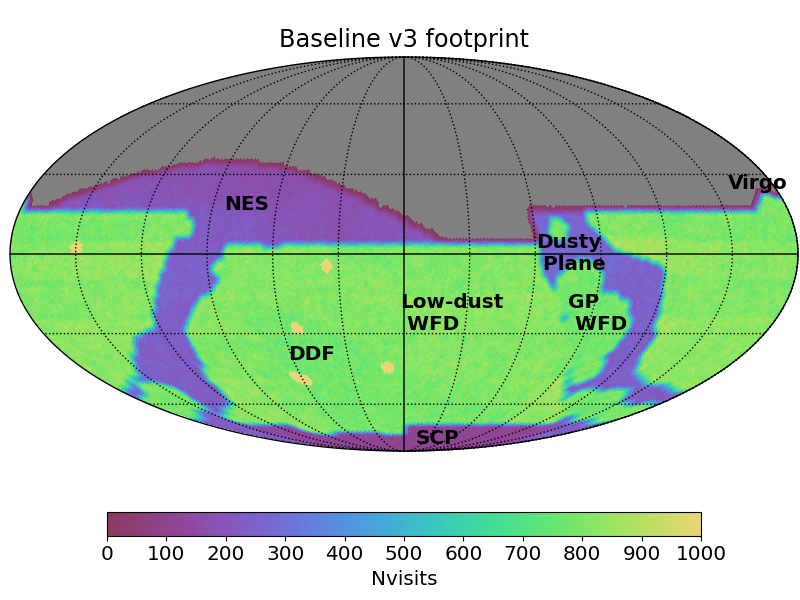
\includegraphics[width=4.7in]{figures/v3footprint.png}
    \caption{Number of visits per pointing in all filters for \texttt{baseline\_v3}. The color bar saturates at 1000. The Virgo cluster is visible on the right of the map, in the Northern hemisphere.%; the DDF fields have $\sim22,000$ visits per field. The Cosmos DDF has almost twice as many.
    }\label{fig:baselinev3Footprint}
\end{figure*}



\setlength\parindent{0.7cm}
\hangindent=0.7cm The footprint follows the description in section~\ref{q:Footprint} above, with the low-dust WFD ranging from a lower limit of Dec $\geq-70\degree$ ---or where the dust extinction exceeds $E(B-V)=0.2$--- to an upper limit of Dec $\leq+15\degree$ for 7~h $\lesssim$ RA $\lesssim$18~h and Dec $\leq+3\degree$ for 0 $\lesssim$ RA $\lesssim$ 7~h and 18~h $\lesssim$ RA $\lesssim$  24~h. The Virgo Cluster, centered on RA$=186.75\degree$, Dec$=12.171$\degree, with a radius of $8.75\degree$, is included in the low-dust WFD footprint. The NES ranges from the upper boundary of the low-dust WFD to $+10\degree$ ecliptic latitude. The SCP covers the remainder of the sphere below the WFD or Galactic Plane region. The Galactic Plane is covered in two parts; WFD-level regions near the Bulge and other regions of interest and a lower level of coverage in the remainder of the regions where dust extinction exceeds $E(B-V)=0.2$.  The median numbers of visits per pointing in these areas over the lifetime of the survey (in any filter) are: 795 visits per pointing in WFD-level areas (the low-dust WFD, Galactic Plane high coverage regions, the Magellanic Clouds, and Virgo cluster), 257 in the high dust extinction (low coverage) Galactic Plane regions, 195 in the NES, and 123 visits per pointing in the SCP. These are split between the $ugrizy$ filters with varying balances in different regions; the NES receives visits only in the $griz$ bands. The total number of visits per pointing is shown in \autoref{fig:baselinev3Footprint}. Evaluation of the footprint and distribution of visits within the Galactic Plane region will continue over the next year.

\hangindent=0.7cm Visits are acquired in $ugrizy$ filters, where $u$ band is available during periods where the lunar illumination is below 40\% and $z$ band is available during periods where the lunar illumination is above 40\% ($u$ and $z$ are swapped, the other filters remain in the camera at all times). Evaluation of this filter swapping procedure compared to alternative swapping strategies, for example alternating $z$ and $y$, will continue over the next year. 

\hangindent=0.7cm In the $u$ band, visits are acquired as a single exposure of 30 seconds to avoid becoming read noise limited; in $grizy$ bands, visits are acquired as a back-to-back set of two 15-second exposures. These 2x15s exposures are less efficient than a single 1x30s visit, due to additional shutter and readout time. During commissioning, 1x30s visits for all bands will be evaluated and, if viable, could be adopted; this would lead to an increase in efficiency of $\sim7\%$. 

\hangindent=0.7cm Visits are generally acquired in pairs separated by approximately 33 minutes. Visits to the same pointing within two hours of the first observation are suppressed at all times, which increases the number of visits that fall into other intervals  and typically pushes a third visit to the following night. Every seventh night, a third visit in the same filter as one of the original pairs is acquired within the same night at an interval of 2--7 hours (randomly assigned per night). These two factors together increase the number of return visits in the same filter during the period of two to 30 hours after the first visit.
Pairs of visits are acquired in different filters, with pairings driven by considerations on sensitivity to sky conditions and availability of filters on the filter wheel; $u$ is paired with $g$ or $r$ band, $g$ is paired with $u$ or $r$ band, $r$ is paired with $u$, $g$ or $i$ band, $i$ is paired with $r$ or $z$ band, $z$ is paired with $i$ or $y$ band, and $y$ is paired with $z$ or $y$ band. The SCOC may engage in further investigation of potential filter pairing strategies. 
\begin{figure*}[t!]
    \centering
    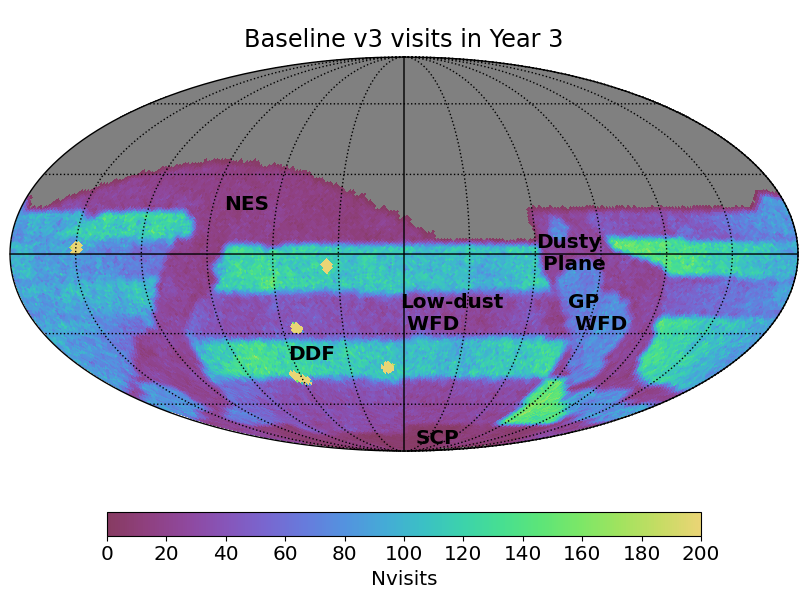
\includegraphics[width=2.5in]{figures/v3footprint_yr3.png}
    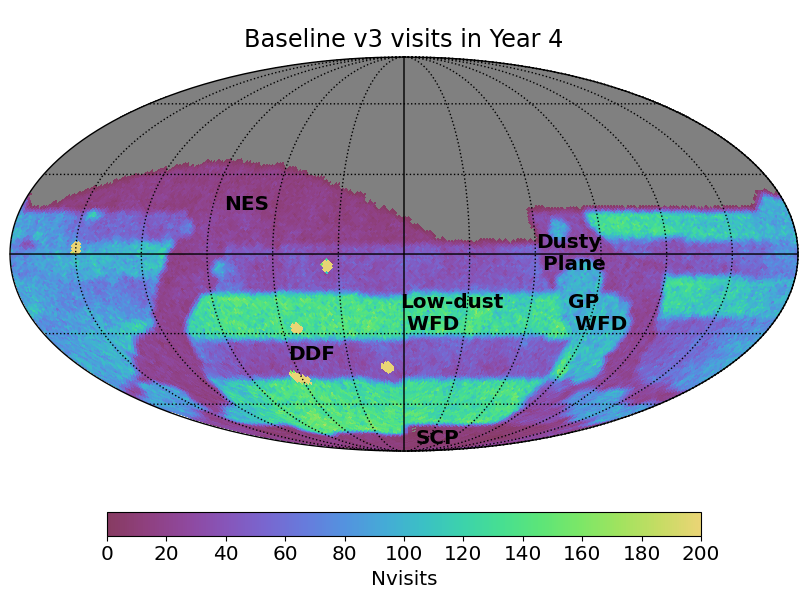
\includegraphics[width=2.5in]{figures/v3footprint_yr4.png}
    \caption{A half-sky rolling cadence is implemented in the low-dust WFD region. Half of the sky is ``active'' and observed at a higher intensity during its visibility season, while half of the sky is ``inactive'' and observed at a lower intensity during this same period. The left panel of this figure shows the visits  collected (in any filter) in (approximately) year 3 of the survey; the right panel shows the visits collected in (approximately) year 4. The central portion of the figure shows the declination bands clearly, as this part of the sky experiences only one observing season during the year selected so that it is strictly ``active'' or ``inactive'' depending on the year.  The outer edges of the low-dust WFD show a fuzzier boundary between the declination bands, as this part of the sky %(especially on the left-hand edge of the NES) 
    experiences both the end of an active season and the start of an inactive season (or vice versa) during this time period. This leads to a more uniform sky coverage. In this simulation, rolling cadence is only implemented in the low-dust WFD, and not the Galactic Plane, NES or SCP. The RA boundary where ``active'' and ``inactive'' declination bands swap after completing a full season is visible in the low-dust WFD region directly (below the ``GP WFD'' label). }\label{fig:baselinev3Rolling}
\end{figure*}

\hangindent=0.7cm A half-sky rolling cadence is implemented in the low-dust WFD, starting $\sim1.5$ years into the survey (when the first part of the sky which has had a complete season of observations in ``uniform'' cadence starts its second season). Four full seasons of rolling occur at each point in the sky, resulting in the last rolling season ending 0.5 years before the end of the survey. The sky is split into four declination bands, so that half of the sky (two bands) are ``active'' at any point in time during the rolling seasons; one of these bands is in the northern portion of the footprint and one in the southern portion, allowing distribution of follow-up requirements over a range of latitudes. An illustration of this rolling cadence, along with additional details, is provided in \autoref{fig:baselinev3Rolling}. The impact of this rolling cadence on the uniformity of the annual data releases will continue to be evaluated. 

\hangindent=0.7cm To generate a templates for the annual data releases, at least 3 to 5 images must be obtained in each bandpass each year on the WFD footprint. Yearly acquisition is desirable to avoid the impact of proper motion in template generation. This places a constraint on the minimum number of images per bandpass  acquired in any year, which is strongest in the $u$ band (as the $u$ band is only targeted to acquire about 50 images per pointing total, this results in $u$ band only minimally rolling; $g$ is only slightly above a similar threshold). 

\hangindent=0.7cm Good seeing visits (seeing $<0.8''$) in $g$, $r$, and $i$ bands are also prioritized in each year. This tends to distribute the best raw atmospheric seeing time into these bands relatively evenly. Due to wavelength-dependent effects on seeing, the resulting $g$ band delivered seeing is slightly worse than the delivered seeing in $r$ and $i$. A goal is set to obtain a minimum of three visits per pointing with delivered seeing $<0.8''$ in each of $gri$ bands.

\hangindent=0.7cm About 6.4\% of the total number of survey visits is devoted to the DDFs. The five DDFs are observed using pre-scheduled observations which are scheduled to ideally space themselves throughout the lunar cycle to optimize both cadence and depth (avoiding the brightest nights or times when the moon is up, for example). Observations for each DDF are acquired in sequences, which are defined as sets of 8 $u$, 10 $g$, 20 $r$, 20 $i$, 24 $z$, and 18 $y$ band 30 second visits (a single 1x30s visit in $u$, 2x15s exposures combined into a visit in $grizy$). As only 5 filters can be in the camera at one time, one of these bandpasses is always missing from the sequence; if the sequence is interrupted by weather or unexpected downtime, or the field becomes unavailable due to pointing constraints, the sequence will be cut short. Sequences that are interrupted or skipped are attempted on following days, but at a lower priority; missed sequences near the ends of seasons where the visibility windows on any night are shorter will tend to be skipped. The median number of visits per pointing for each of the DDFs is on the order of $10,000$, with the exception of the COSMOS field which receives almost $19,000$ visits. Following the recommendation in \autoref{q:DDF}, COSMOS is scheduled to achieve 10-year depth ($\sim10,000$ visits) by the end of year 3. It then continues to acquire observations at the same rate as the other DDF fields. The EDFS is split into two pointings; each pointing receives $\sim6,600$ visits. Generally, coadded DDF depths are about 1.3 magnitudes deeper in each bandpass than the coadded depth of a WFD pointing in the same bandpass. Dithering is implemented for each of the DDFs, with maximum offsets $\sim0.7\degree$ (the size of a raft). Optimization of the DDF scheduling is expected to continue through 2023.

\hangindent=0.7cm The near-sun twilight NEO microsurvey is implemented as recommended in \autoref{q:Micro}. Every fourth night during morning and evening twilight, visits are acquired in sets of four at low-solar elongations, separated by $\sim5$ minutes, with single exposure 15s visits in $r$, $i$, and $z$ bands. These visits are necessarily in high-airmass fields, which, as a side-effect, extends the season length for regions within this footprint (although with somewhat shallower visits). The NEO microsurvey footprint is shown in \autoref{fig:baselinev3Micro}.

\begin{figure*}[t!]
    \centering
    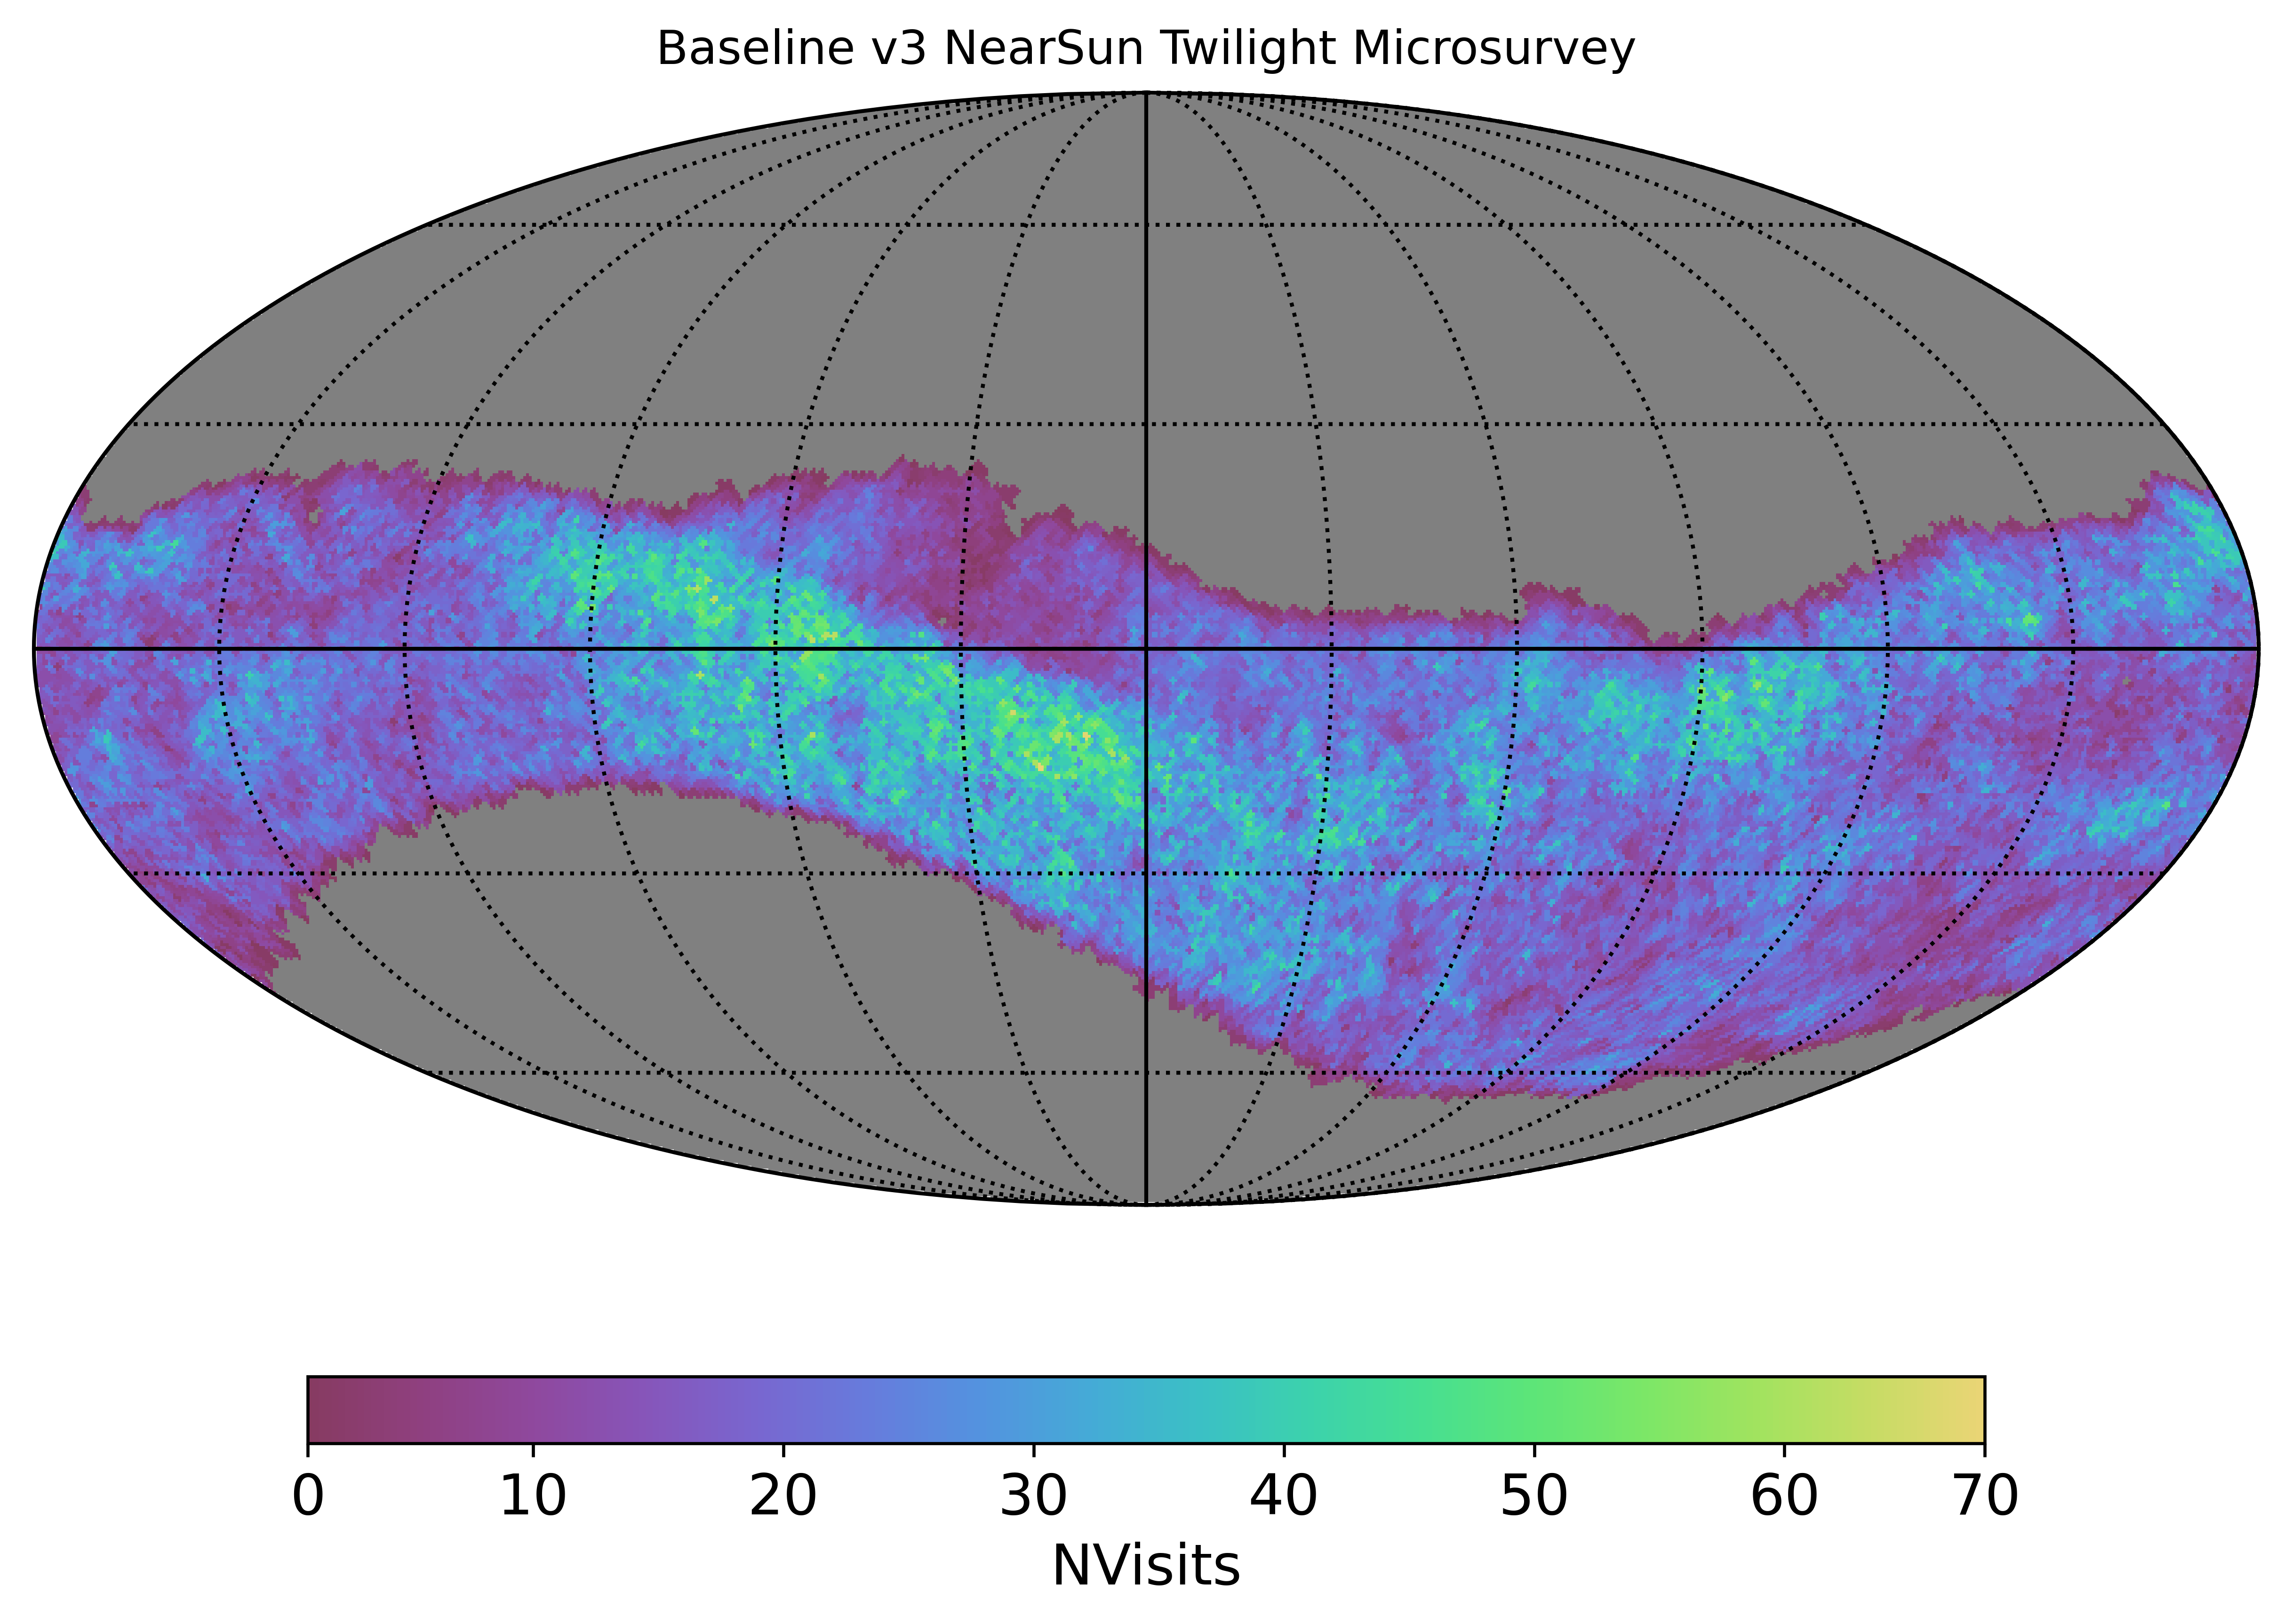
\includegraphics[width=4.7in]{figures/v3TwilightMicrosurvey.png}
    \caption{The footprint of the near-sun NEO twilight microsurvey. This microsurvey executes every fourth night in morning and evening twilight, with a footprint defined by solar elongation with $<=60\degree$ and airmass $X<=2$ limits, and regions with Dec $<= 30\degree$ and ecliptic latitude $< 40\degree$. Within the twilight period, four 15s visits separated by about five minutes are attempted. These areas of the sky are only visible for a short period; linking within a given night aids the discovery of near-sun asteroids. }\label{fig:baselinev3Micro}
\end{figure*}